\chapter{Vybrané zbernicové protokoly}
\label{kap:zbernice}

V tejto kapitole stručne spomenieme vybrané zbernicové protokoly a zhrnieme ich kľúčové vlastnosti, ktoré budú relevantné v ďalších častiach práce. Vo všeobecnosti existuje mnoho rôznych zbernicových protokolov. Tie môžu využívať rôzne techniky, ktoré umožňujú zabezpečiť komunikáciu a jej riadenie. Mnoho týchto protokolov má však veľa spoločných znakov. Aj preto sa v práci budeme venovať iba niektorým vybraným. V tejto kapitole najskôr uvedieme niektoré základné vlastnosti zberníc. Následne predstavíme 3 príklady zberníc (UART, SPI, I\textsuperscript{2}C). Podporu pre UART a SPI zároveň implementujeme na FPGA MITM obvode popísanom v kapitole \ref{kap:implementacia}.

\section{Vlastnosti hardvérových zberníc}
V tejto časti spomenieme vybrané vlastnosti hardvérových zberníc a základnú kategorizáciu na základe týchto vlastností. Vlastnosti, ktoré opíšeme sú relevantné pre spôsob implementácie hardvérového MITM útoku na danej zbernici. Vlastnosti, ktoré nie sú relevantné, nebudeme popisovať.

\subsection{Synchrónne a asynchrónne zbernice} \label{sek:syncAsync}
Pre účel MITM útoku je veľmi dôležité rozlišovať medzi tzv. synchrónnymi a asynchrónnymi zbernicami. Synchrónne zbernice sa vyznačujú tým, že dátový signál je doplnený o~synchronyzačný hodinový signál, ktorý riadi prenos dát na zbernici a umožňuje správne dekódovať prenášané dáta. Takýto signál môže byť explicitne vysielaný na samostatnej linke, napr. zbernice SPI \cite{spiBus} a I\textsuperscript{2}C \cite{i2cSpec}. Tento spôsob synchronizácie je znázornený na obrázku \ref{obr:clockDemo}.

\begin{figure}
    \centerline{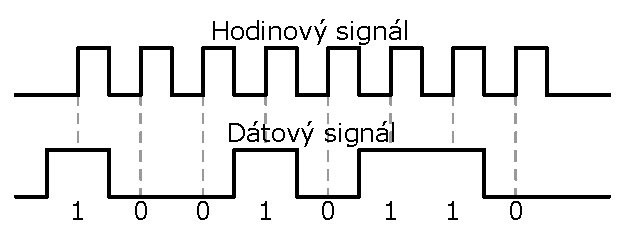
\includegraphics[width=1\textwidth]{images/signals/clockDemo.pdf}}
    \caption[Príklad synchrónneho prenosu dát]{Príklad synchrónneho prenosu dát. V príklade na obrázku sú jednotlivé bity čítané pri nábehovej hrane hodinového signálu (zvislé čiary).}
    \label{obr:clockDemo}
\end{figure}

Iný spôsob ako preniesť hodinový signál je zakódovať hodinový signál vrámci dátového. Prijímajúce zariadenie dokáže následne z prijatého signálu správne dekódovať synchronizované dáta. Tento spôsob synchrónneho prenosu dát sa využíva najmä pri vysokorýchlostných (angl. high-speed) sériových zberniciach \cite{serdes}, tzv. SerDes (Serializer-Deserializer), ako sú napríklad USB \cite{usbSpec} a PCIe \cite{pcieSpec}. Vysokorýchlostným zberniciam sa v práci nebudeme venovať, nakoľko si na fyzickej vrstve vyžadujú dedikovaný hardvér a~vrámci FPGA obvodov sa zvyknú implementovať iba vyššie vrstvy daných protokolov.

Protikladom synchrónnych zberníc sú asynchrónne zbernice. Rozdiel spočíva v tom, že hodinový signál je implicitný a je daný parametrom protokolu, zvyčajne nazývaný symbolová rýchlosť (angl. baud rate). Symbolová rýchlosť určuje počet prenesených symbolov (napr. bitov) za sekundu. Príkladom takejto zbernice je UART \cite{uartBus}.

Z pohľadu MITM útoku nie je podstatné rozlišovať medzi asynchrónnymi zbernicami a synchrónnymi so zabudovaným hodinovým signálom. Ich spoločným znakom je, že nemáme explicitný hodinový signál, ktorý by riadil komunikáciu. To umožňuje v niektorých prípadoch odchytiť celý odvysielaný rámec, spracovať ho a následne odvysielať. V prípade synchrónnej zbernice s explicitným hodinovým signálom môže byť pozastavenie nemožné. Protokol danej zbernice určuje, ktorá strana má generovať riadiaci hodinový signál. V prípade, že hodinový signál generuje druhá strana, falošné dáta musíme vysielať synchrónne s týmto signálom. Tento problém úzko súvisí s tzv. master-slave architektúrou, ktorú popíšeme v ďalšej časti.

\subsection{Architektúra master-slave} \label{sek:masterSlave}
Veľká časť protokolov hardvérových zberníc je postavená na asymetrickej master-slave architektúre. V master-slave architektúre protokol definuje (zvyčajne jedno) zariadenie, ktoré riadi komunikáciu na zbernici, tzv. master. Riadenie komunikácie môže znamenať riadenie prístupu ku zbernici, vysielanie hodinového signálu v prípade synchrónnej zbernice a pod. Spôsob riadenia sa môže líšiť v závislosti od protokolu. Ostatné zariadenia, nazývané slave, sa musia riadeniu prispôsobiť. Okrem iného, to zvyčajne znamená, že môžu vysielať dáta len v časových intervaloch vyhradených master stranou. Príkladom master-slave zberníc sú SPI \cite{spiBus}, I\textsuperscript{2}C \cite{i2cSpec} a USB \cite{usbSpec}. Niektoré zbernice, napr. I\textsuperscript{2}C \cite{i2cSpec}, podporujú aj tzv. multi-master architektúru, ktorá umožňuje mať viacero master zariadení pripojených ku zbernici súčasne. Takýmto scenárom sa v práci nebudeme venovať, nakoľko ich využitie je pomerne zriedkavé.

Pre MITM útok prináša master-slave architektúra značné komplikácie. Najmä na master strane (rozhranie, na ktorom MITM zariadenie simuluje skutočné slave zariadenie) predstavuje principiálny problém fakt, že falošné dáta, ktoré chceme poslať musíme odvysielať vo vyhradených časových intervaloch určených mastrom. Toto obmedzenie je problematické v prípade ak falošné dáta závisia od dát vyslaných druhou stranou, ktoré sme ešte neprijali. V kapitole \ref{kap:implementacia}, časti \ref{sek:spiImplementation}, uvedieme čiastočné riešenie na tento problém. Asymetrickosť master-slave architektúry však znamená, že už na úrovni MITM logiky je potrebné poznať, ktorá strana je master a ktorá slave, čo principiálne znemožňuje úplne abstrahovať od tejto vlastnosti.

\subsection{Ďalšie vlastnosti zberníc}
Existuje aj mnoho ďalších vlastností, na základe ktorých môžeme zbernice kategorizovať. Tie nie sú až tak relevantné pre MITM útoky, no môžu ovplyvniť spôsob jeho implementácie, preto niektoré stručne spomenieme.

Na základe smeru komunikácie rozlišujeme medzi simplex, half-duplex a full-duplex zbernicami. Simplex zbernice umožňujú iba jednosmernú komunikáciu. Dnes sú pomerne zriedkavé, zvyknú sa používať na zapojenie niektorých senzorov, ktoré podporujú iba jednosmernú komunikáciu. Príkladom simplex zbernice môže byť zbernica UART \cite{uartBus}, ktorá je štandardne full-duplex, ale umožňuje aj zapojenie v simplex režime. Half-duplex zbernice podporujú obojsmernú komunikáciu, pričom jednotlivé strany nemôžu vysielať súčasne. Príkladmi half-duplex zbernice sú I\textsuperscript{2}C \cite{i2cSpec} a 1-Wire \cite{1wireBus}. Full-duplex zbernice umožňujú komunikáciu oboma smermi súčasne, napr. UART \cite{uartBus} v štandardnom zapojení, SPI \cite{spiBus}, USB \cite{usbSpec} a PCIe \cite{pcieSpec}.

Ďalej rozlišujeme medzi sériovými a paralelnými zbernicami. Sériové sa vyznačujú tým, že jednotlivé symboly sú prenášané sériovo, pričom niektoré zbernice, napr. PCIe \cite{pcieSpec}, podporujú sériový prenos viacerých rámcov súčasne po paralelných linkách. Paralelné zbernice naopak prenášajú samotný rámec paralelne po viacerých linkách.

Posledné dve kategórie, ktoré uvedieme sú point-to-point zbernice a multi-drop zbernice. Point-to-point zbernice sú určené pre zapojenie práve dvoch zariadení a sú následne dedikované pre prenos dát medzi týmito dvoma zariadeniami. Príkladmi point-to-point zberníc sú UART \cite{uartBus} a PCIe \cite{pcieSpec}. Multi-drop zbernice naopak podporujú zapojenie viacej ako dvoch zariadení súčasne. Následne je potom potrebné v rámci komunikácie jednoznačne určiť zariadenie, pre ktoré sú vysielané dáta určené. Najčastejším spôsobom je adresácia, napr. I\textsuperscript{2}C \cite{i2cSpec} a USB \cite{usbSpec}. Iný spôsob môže byť tzv. slave-select, označovaný aj chip-select, ktorý sa používa napríklad pri zbernici SPI \cite{spiBus}. Vizuálne zhrnutie spomenutej kategorizácie zberníc je na obrázku \ref{obr:busTree}.

\begin{figure}
    \centerline{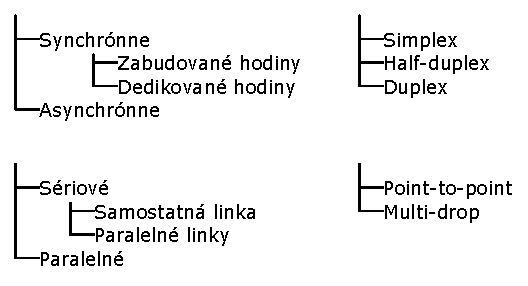
\includegraphics[width=1\textwidth]{images/misc/busTree.pdf}}
    \caption[Vybrané kategórie zberníc]{Vybrané kategórie zberníc.}
    \label{obr:busTree}
\end{figure}

\section{UART zbernica}
UART (Universal Asynchronous Receiver Transmitter) je defakto-štandard, ktorý okrem hardvérového rozhrania definuje aj komunikačný protokol a niektoré jeho parametre. Z hľadiska kategorizácie ide o sériovú full-duplex asynchrónnu point-to-point linku. Keďže ide o point-to-point linku, riadenie prístupu nie je potrebné.

\subsection{Hardvér UART zbernice}
UART zbernica pozostáva z dvoch hlavných liniek: RX (Receive) pre prijímanie dát a~TX (Transmit) pre vysielanie dát. Okrem týchto dátových existujú aj niektoré ďalšie riadiace linky, ktoré sú súčasťou RS-232 štandardu \cite{rs232Spec} (ktorý využíva UART protokol), tie sa dnes zriedka využívajú, preto ich zanedbáme. Schéma zapojenia UART zbernice medzi dvoma zariadeniami je na obrázku \ref{obr:uartWiring}.

\begin{figure}
    \centerline{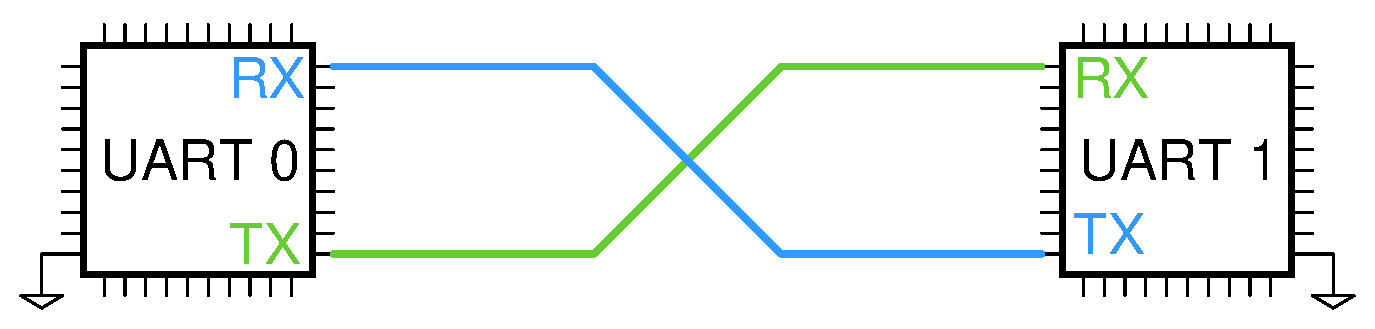
\includegraphics[width=0.9\textwidth]{images/busses/uartWiring.pdf}}
    \caption[Zapojenie zbernice UART]{Zapojenie zbernice UART. Linky RX a TX sú zapojené do kríža.}
    \label{obr:uartWiring}
\end{figure}

\subsection{UART protokol a štruktúra rámcov}
UART definuje aj komunikačný protokol pre posielanie dát. V pasívnom stave je napätie danej linky na úrovni logickej 1 (zvyčajne 3.3\,V alebo 5\,V). Vysielaný rámec vždy začína bitom s logickou hodnotou 0, tzv. START bit.  Nasledujú samotné dáta (počnúc najmenej významným bitom), pričom počet bitov sa môže líšiť v závislosti od nastavených parametrov, najčastejšie 8 bitov. Za dátovými bitmi môže nasledovať nepovinný paritný bit, ten sa zriedka využíva. Rámec je vždy ukončený tzv. STOP bitom s logickou hodnotou 1. Za STOP bitom môže nasledovať ľubovoľná pauza, ktorá sa v~literatúre označuje aj predĺžený STOP bit. Štruktúra UART rámca je znázornená na obrázku \ref{obr:uartFrame}.

\begin{figure}
    \centerline{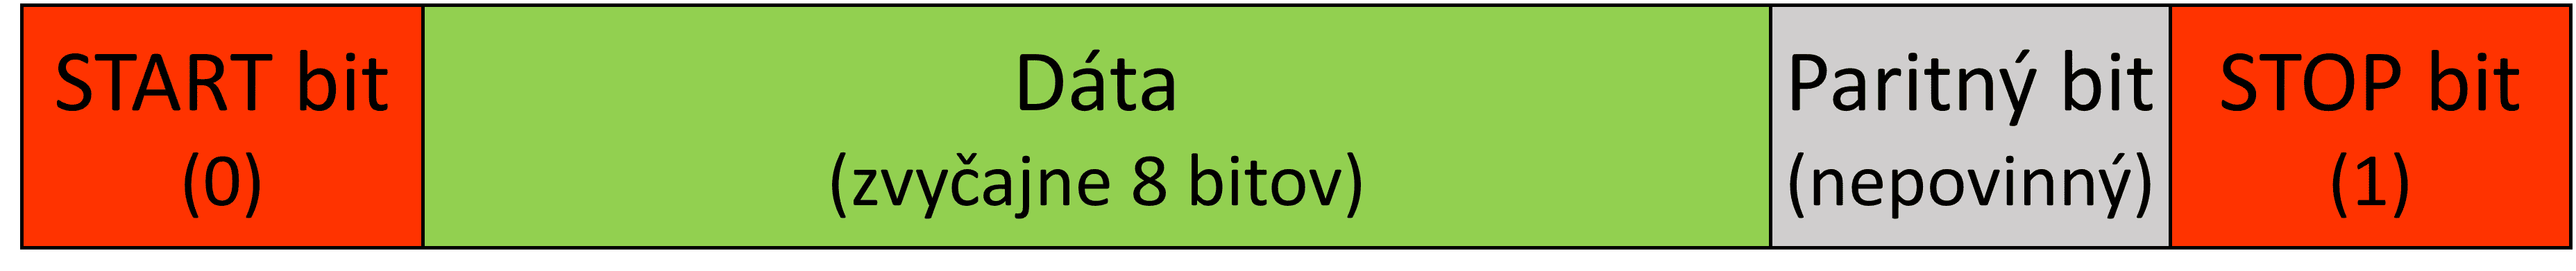
\includegraphics[width=1\textwidth]{images/busses/uartFrame.png}}
    \caption[Štruktúra UART rámca]{Štruktúra UART rámca. Dáta sú posielané od najmenej významného bitu.}
    \label{obr:uartFrame}
\end{figure}

UART je asynchrónna zbernica, preto dĺžka trvania jedného bitu je určená implicitne, symbolovou rýchlosťou. Princíp sme spomenuli v časti \ref{sek:syncAsync}. Dve najčastejšie používané hodnoty symbolovej rýchlosti na zbernici UART sú 115\,200 a 9\,600 symbolov za sekundu.

\section{SPI Zbernica}
Zbernica SPI je defakto-štandard, ktorý definuje hardvérové rozhranie, pre zapojenie komunikujúcich strán. SPI je synchrónna sériová zbernica typu multi-drop s explicitným hodinovým signálom na dedikovanej linke. Keďže ide o defakto-štandard, zbernica SPI nedefinuje predpísanú štruktúru posielaných dát \cite{spiBus}.

\subsection{Riadenie prístupu k zbernici}
Komunikácia na SPI zbernici je riadená master-slave architektúrou. Prístup k zbernici riadi master prostredníctvom dedikovanej linky SS (Slave Select) pre každé slave zariadenie. Linky SS zvyknú byť označené aj ako CS (Chip Select). V pasívnom stave je na každom SS vodiči napätie na úrovni logickej 1 (napr. 3.3\,V alebo 5\,V). Pred začatím komunikácie s vybraným slave zariadením nastaví master logickú hodnotu 0 (napätie 0\,V) na príslušnom SS vodiči, čím umožní komunikáciu medzi mastrom a~príslušným slave zariadením. V niektorých implementáciách je polarita SS liniek invertovaná. Tento spôsob riadenia zbernice vytvára ilúziu point-to-point linky medzi komunikujúcimi stranami, preto v zbernici SPI nie je potrebná adresácia.

\subsection{Hardvér SPI zbernice}
SPI zbernica pozostáva z troch hlavných liniek: MISO (Master In Slave Out), ktorá zabezpečuje prenos dát smerom od slave zariadení k master zariadeniu, MOSI (Master Out Slave In) pre prenos dát opačným smerom a SCLK (Serial Clock) pre prenos hodinového signálu (generovaný master zariadením) \cite{spiBus}. Schéma zapojenia pomocou SPI zbernice je na obrázku \ref{obr:spiWiring}. Dáta po vodičoch MISO a MOSI môžu tiecť súčasne čo umožňuje full-duplex komunikáciu.

\begin{figure}
    \centerline{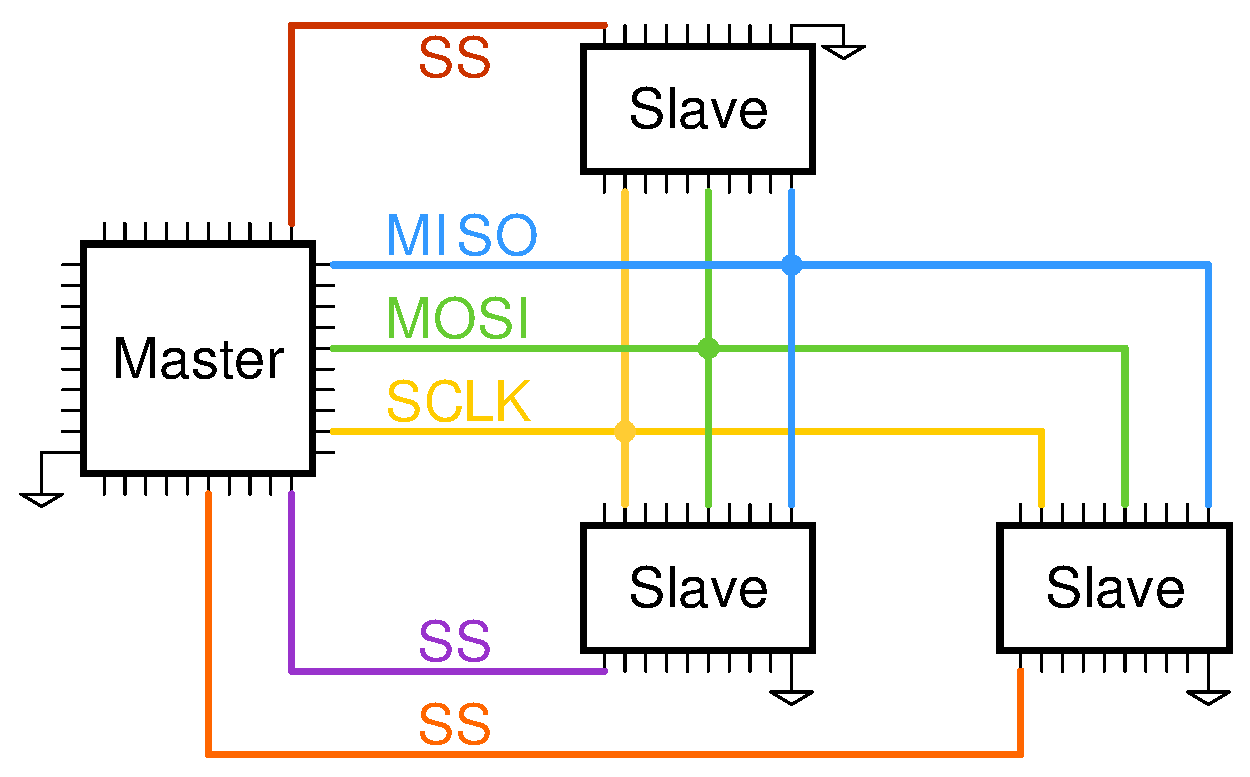
\includegraphics[width=1\textwidth]{images/busses/spiWiring.pdf}}
    \caption[Zapojenie zbernice SPI]{Zapojenie zbernice SPI.}
    \label{obr:spiWiring}
\end{figure}

Existujú štyri spôsoby, tzv. módy, ktorými hodinový signál riadi prenos dát na zbernici a líšia sa kombináciou dvoch parametrov. Prvým parametrom je polarita hodín (CPOL), ktorý určuje, či je v pasívnom stave úroveň napätia hodinového signálu na úrovni logickej 0 alebo 1. Druhý parameter je fáza hodín (CPHA). Ten rozhoduje, na ktorej hrane sa dáta čítajú. Vizualizácia všetkých štyroch režimov je na obrázku \ref{obr:spiModes}. Výber módu závisí od implementácie SPI na jednotlivých zariadeniach, veľa zariadení podporuje iba mód 0 -- polarita v pasívnom stave 0 a čítanie na nábehovej hrane, preto sa v práci budeme zaoberať iba touto konfiguráciou.

\begin{figure}
    \centerline{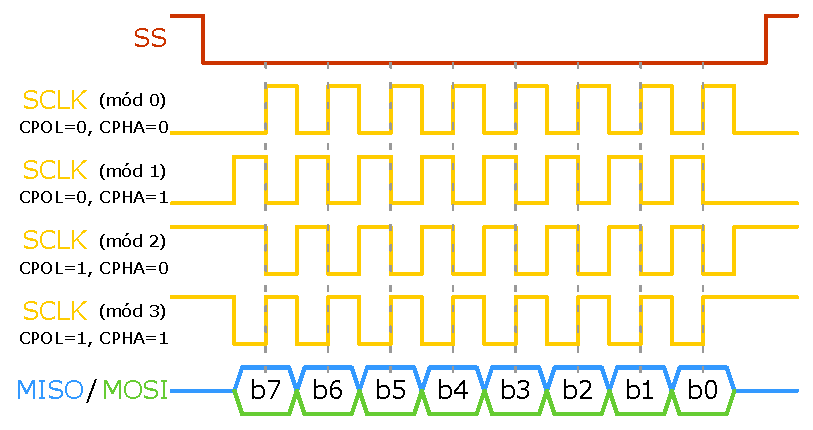
\includegraphics[width=0.9\textwidth]{images/busses/spiClocks.pdf}}
    \caption[Režimy hodín zbernice SPI]{Režimy hodín zbernice SPI. Zvislé čiary znázorňujú hrany hodinového signálu, pri ktorých sa čítajú dáta na linkách MISO a MOSI.}
    \label{obr:spiModes}
\end{figure}

\section{I\textsuperscript{2}C zbernica}
I\textsuperscript{2}C (Inter-Integrated Circuit) je štandardizovaná zbernica, vyvinutá spoločnosťou Philips Semiconductors, určená pre jednoduchú komunikáciu medzi integrovanými obvodmi \cite{i2cSpec} väčšinou v rámci jednej dosky plošných spojov. Podobne ako SPI, I\textsuperscript{2}C je synchrónna sériová zbernica typu multi-drop s dedikovaným hodinovým signálom. Narozdiel od UART a SPI zberníc I\textsuperscript{2}C podporuje iba half-duplex komunikáciu.

\subsection{Hardvér I\textsuperscript{2}C zbernice}
Zbernica pozostáva z dvoch vodičov: SDA (Serial Data Line), ktorý zabezpečuje sériový prenos dát (bitov) a SCL (Serial Clock Line) pre prenos synchronizačného hodinového signálu \cite{i2cSpec}. Vodiče sú na komunikujúcich zariadeniach pripojené v tzv. open-drain režime a každé zvlášť sú cez zdvíhací odpor (angl. pull-up rezistor) pripojené k napätiu 5\,V resp. 3.3\,V v závislosti od konfigurácie. Na obrázku \ref{obr:i2cWiring} je znázornené zapojenie zariadení pomocou zbernice I\textsuperscript{2}C.

\begin{figure}
    \centerline{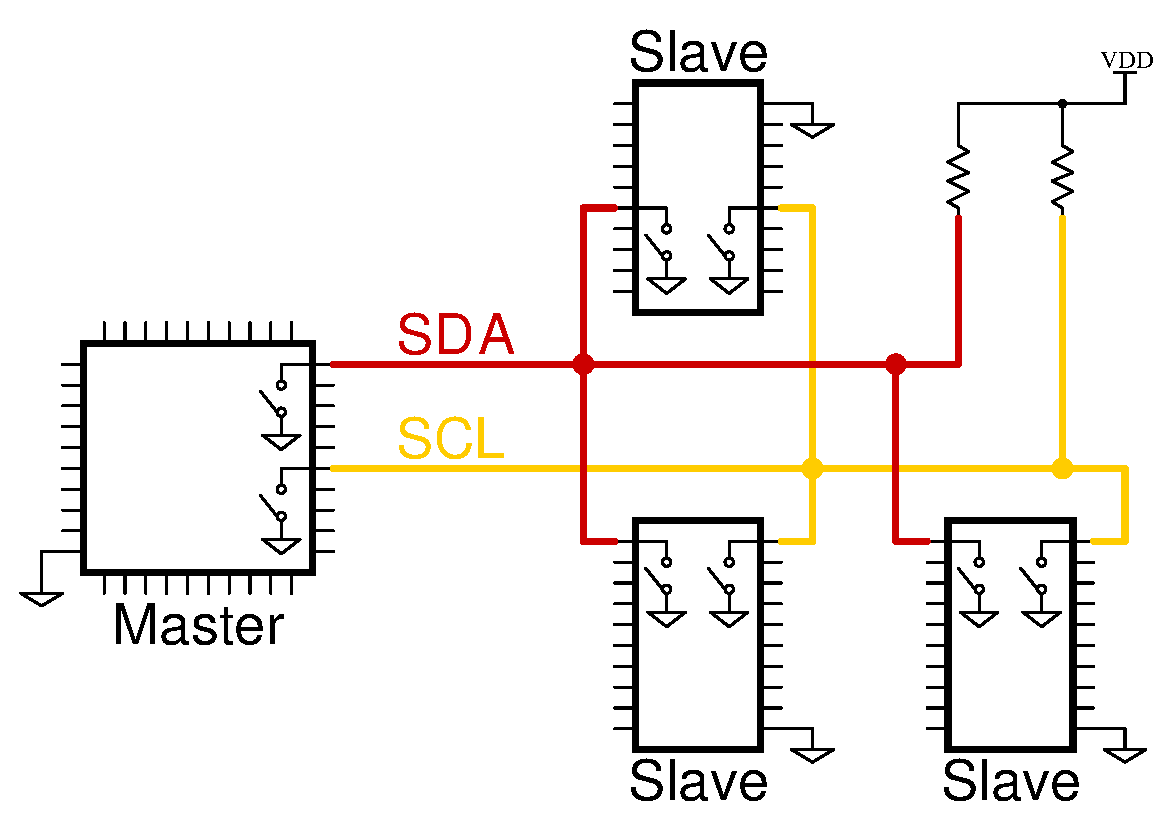
\includegraphics[width=0.9\textwidth]{images/busses/i2cWiring.pdf}}
    \caption[Zapojenie zbernice I\textsuperscript{2}C]{Zapojenie zbernice I\textsuperscript{2}C. Open-drain logika interného zapojenia vodičov v~zariadeniach je znázornená pomocou \uv{spínačov}. V skutočnosti je realizovaná pomocou tranzistorov.}
    \label{obr:i2cWiring}
\end{figure}

V pasívnom stave je teda na vodičoch hodnota napätia 5\,V (resp. 3.3\,V), čo na dátovej linke zodpovedá logickej hodnote 1. V prípade, že práve vysielajúce zaradenie chce poslať bit s logickou hodnotou 0, \uv{pripojí} (napr. pomocou tranzistora) vodič na spoločnú zem, čím napätie klesne na 0\,V. Dáta na vodiči SDA sú vzorkované pri nábehovej hrane na SCL signálovej linke \cite{i2cSpec}.

\subsection{Riadenie prístupu k zbernici}
Komunikácia na I\textsuperscript{2}C zbernici je riadená architektúrou master-slave \cite{i2cSpec}. Master zariadenie riadi komunikáciu na hardvérovej aj protokolovej úrovni. Na hardvérovej úrovni master zariadenie určuje rýchlosť komunikácie generovaním hodinových impulzov na SCL linke. Zbernica podporuje rôzne konfigurácie, ktoré sa líšia rýchlosťou rádovo od 100\,kbps až po niekoľko\,Mbps. Na protokolovej úrovni je každá komunikácia iniciovaná aj ukončená master zariadením a slave zariadenia musia synchrónne posielať dáta vo vyhradených časoch, ktoré definuje protokol.

Zariadenie, s ktorým chce master komunikovať je určené adresáciou. Každé slave zariadenie má pridelenú 7-bitovú (resp. 10-bitovú v novšej verzii štandardu) adresu, ktorá je zvyčajne pevne nastavená výrobcom hardvéru \cite{i2cSpec}. Z dôvodu predchádzania kolízií v adresách, zvyknú výrobcovia prideliť zariadeniu viacero adries, z ktorých je možne nakonfigurovať práve jednu, väčšinou hardvérovým spínačom.

\subsection{Protokol a štruktúra rámcov}
I\textsuperscript{2}C štandard striktne definuje spôsob komunikácie na zbernici. Samotná komunikácia vyzerá nasledovne: Master zariadenie nastaví úroveň napätia na SDA linke na hodnotu logickej 0, čím pošle tzv. START bit, ktorý signalizuje začiatok komunikácie. Nasleduje 7-bitová (resp. 10-bitová) adresa zariadenia, s ktorým chce master komunikovať, počnúc najvýznamnejším bitom adresy. Za adresou nasleduje jeden tzv. R/W bit, ktorý označuje, či ide o operáciu čítania alebo zápisu z pohľadu master strany (1 predstavuje čítanie, 0 predstavuje zápis). S nasledujúcim hodinovým impulzom musí adresované slave zariadenie komunikáciu potvrdiť (pošle tzv. ACK bit) tým, že úroveň napätia na SDA linke nastaví na hodnotu logickej 0. Potom nasledujú samotné dáta, ktoré posiela master (resp. slave v prípade, že ide o~operáciu čítania). Dáta sú členené na 8-bitové sekvencie, ktoré sú zakaždým potvrdzované druhou stranou rovnakým spôsobom a tiež sú posielané v poradí od najvýznamnejšieho bitu. Za posledným potvrdením dát pošle master tvz. STOP bit (napätie ponechá na úrovni logickej 1), čím signalizuje ukončenie komunikácie. Štruktúra rámca je znázornená na obrázku \ref{obr:i2cFrame}.

\begin{figure}
    \centerline{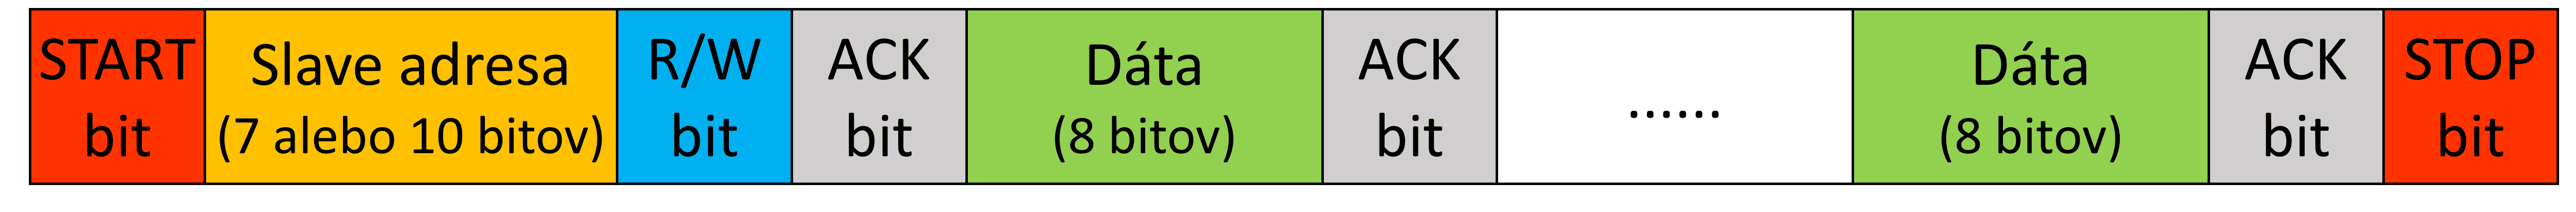
\includegraphics[width=1\textwidth]{images/busses/i2cFrame.png}}
    \caption[Štruktúra I\textsuperscript{2}C rámca]{Štruktúra I\textsuperscript{2}C rámca. Adresa aj dáta sú posielané od najvýznamnejšieho bitu.}
    \label{obr:i2cFrame}
\end{figure}

V prípade, že počas komunikácie nastane chyba, prijímajúce zariadenie nepošle ACK bit. Teda napätie na SDA linke ostane na úrovni logickej 1 (tzv. NACK bit), čo je zároveň pasívny stav. V takomto prípade môže master reagovať dvoma spôsobmi. Buď pošle STOP bit, čo znamená okamžité ukončenie komunikácie, alebo môže zopakovať komunikáciu od začiatku, tým, že pošle START bit. Postupnosť NACK a STOP môže byť master zariadením zároveň využitá na signalizáciu ukončenia komunikácie v prípade operácie čítania \cite{i2cSpec}.

\subsection{Mechanizmus naťahovania hodín}
Naťahovanie hodín (angl. clock stretching) je mechanizmus I$^2$C protokolu, ktorý umožňuje slave zariadeniu dočasne spomaliť hodinové impulzy generované master zariadením \cite{i2cSpec}. To umožňuje slave zariadeniu spomaliť rýchlosť komunikácie, v prípade potreby väčšieho času pre spracovanie dát.

Počas prebiehajúcej komunikácie master zariadenie monitoruje vysielaný hodinový signál na SCL linke. Pripomíname, že vodič SCL linky je pripojený cez zdvíhací odpor k zdroju napätia a zariadenia majú vodič pripojený v open-drain režime. Pokiaľ chce slave zariadenie spomaliť komunikáciu môže podržať SCL vodič pripojený na zem, čím dosiahne efekt, že napätie na vodiči ostane na úrovni logickej 0 aj v prípade, že master posiela logickú 1. Tento stav dokáže master detegovať a následne prispôsobiť rýchlosť komunikácie -- dáta sa čítajú na nábehovej hrane hodín, preto bude vysielanie aktuálneho bitu predĺžené. Mechanizmus naťahovania hodín je znázornený na obrázku~\ref{obr:i2cStretch}.

\begin{figure}
    \centerline{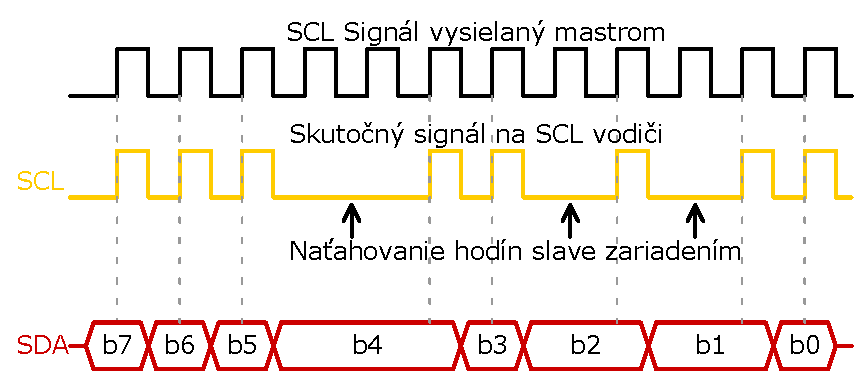
\includegraphics[width=0.9\textwidth]{images/busses/i2cStretch.pdf}}
    \caption[Mechanizmus naťahovania hodín]{Mechanizmus naťahovania hodín. Zvislé čiary znázorňujú skutočné nábehové hrany na SCL vodiči, pri ktorých sa čítajú jednotlivé bity na SDA vodiči.}
    \label{obr:i2cStretch}
\end{figure}